\documentclass[10pt,pdftex]{beamer}

\usepackage{graphicx}
\mode<presentation>
{
  \usetheme{Darmstadt}

  \usecolortheme{seahorse}
  \usecolortheme{rose}
}

\usepackage[latin1]{inputenc} 
\usepackage{amsmath}
\usepackage{amsfonts}
\usepackage{url}

\usepackage{listings, bera}  
\lstset{language=C,  
   commentstyle=\color{comments}\emph,
   }  

\lstset{
  showstringspaces=false
}
\lstset{xleftmargin=0.2cm, xrightmargin=0.2cm}
\lstset{language=bash}

\lstset{breaklines=true}



\setbeamercovered{
  still covered={\opaqueness<1->{10}},
  again covered={\opaqueness<1->{75}}
}

\title{MPI wrapper}
\subtitle{}
\author{Paul M�ller}

\begin{document}

\AtBeginSection[]
{
   \begin{frame}
       \frametitle{Content}
       \tableofcontents[currentsection]
   \end{frame}
}

\maketitle

\begin{frame} 
  \begin{block}{}
    \tableofcontents
  \end{block}
\end{frame}



\section{MPI Wrapper}
\subsection{Purpose}

\begin{frame}
  \begin{block}{Purpose}
    Trace the essential parts of the execution of an MPI program.
  \end{block}
\end{frame}

\subsection{Goals}

\begin{frame}
  \begin{block}{Purpose}
    Trace the essential parts of the execution of an MPI program.
  \end{block}
  \begin{block}{Goals}
    \begin{itemize}
    \item Human-readable xml output
    \item usable with Open MPI and MPICH
    \item primary use: PIOsim
    \item no interference with the program's MPI communication
    \end{itemize}
  \end{block}
\end{frame}

\begin{frame}
  \begin{block}{Purpose}
    Trace the essential parts of the execution of an MPI program.
  \end{block}
  \begin{block}{What is essential?}
    \begin{itemize}
    \item Function calls
    \item Interaction information (communicators, tags)
    \item Timing (or ``computation time'')
    \item Datatypes $\rightarrow$ transmission size
    \item Files
    \end{itemize}
  \end{block}
  \begin{block}{optional}
    \begin{itemize}
    \item nested calls
    \end{itemize}
  \end{block}
  \begin{block}{Not important}
    \begin{itemize}
    \item actual data
    \item program logic
    \end{itemize}
  \end{block}
\end{frame}

\begin{frame}
  \begin{block}{local data}
    \begin{itemize}
    \item Function calls
    \item \emph{Time}
    \end{itemize}
    Local logging; no further modification of logfile
  \end{block}

  \begin{block}{shared data}
    \begin{itemize}
    \item Files
    \item MPI communicators
    \item \emph{Datatypes}
    \end{itemize}
  Local logging; Data is assembled during postprocessing
  \end{block}
\end{frame}

\subsection{Trace Format}

\begin{frame}[fragile]
  \begin{block}{Files that compose the trace}
    \begin{itemize}
    \item program\_node01\_0\_0.trc ... program\_node03\_9\_0.trc
    \item program.proj
    \end{itemize}
  \end{block}

  \begin{block}{.trc files}
    \begin{itemize}
    \item local data
    \item naming:
\begin{lstlisting}
<program name>_<hostname>_<rank>_<thread>.trc
\end{lstlisting}
    \end{itemize}
  \end{block}

  \begin{block}{.proj files}
    \begin{itemize}
    \item which files belong to the trace
    \item which resources are used
    \item naming:
\begin{lstlisting}
<program name>.proj
\end{lstlisting}
    \end{itemize}
  \end{block}
\end{frame}

\section{Components}
\subsection{Overview}

\begin{frame}
  \begin{block}{}
    \begin{description}
    \item[HDTraceWritingCLibrary] Writing formatted log files 
      (in collaboration with Stephan Krempel)
    \item[HDMPIwrapper] intercepting MPI calls
    \item[Project Description Merger] Generate a project description
      from individual trace files
    \end{description}
  \end{block}
\end{frame}

\begin{frame}
  \begin{block}{}
    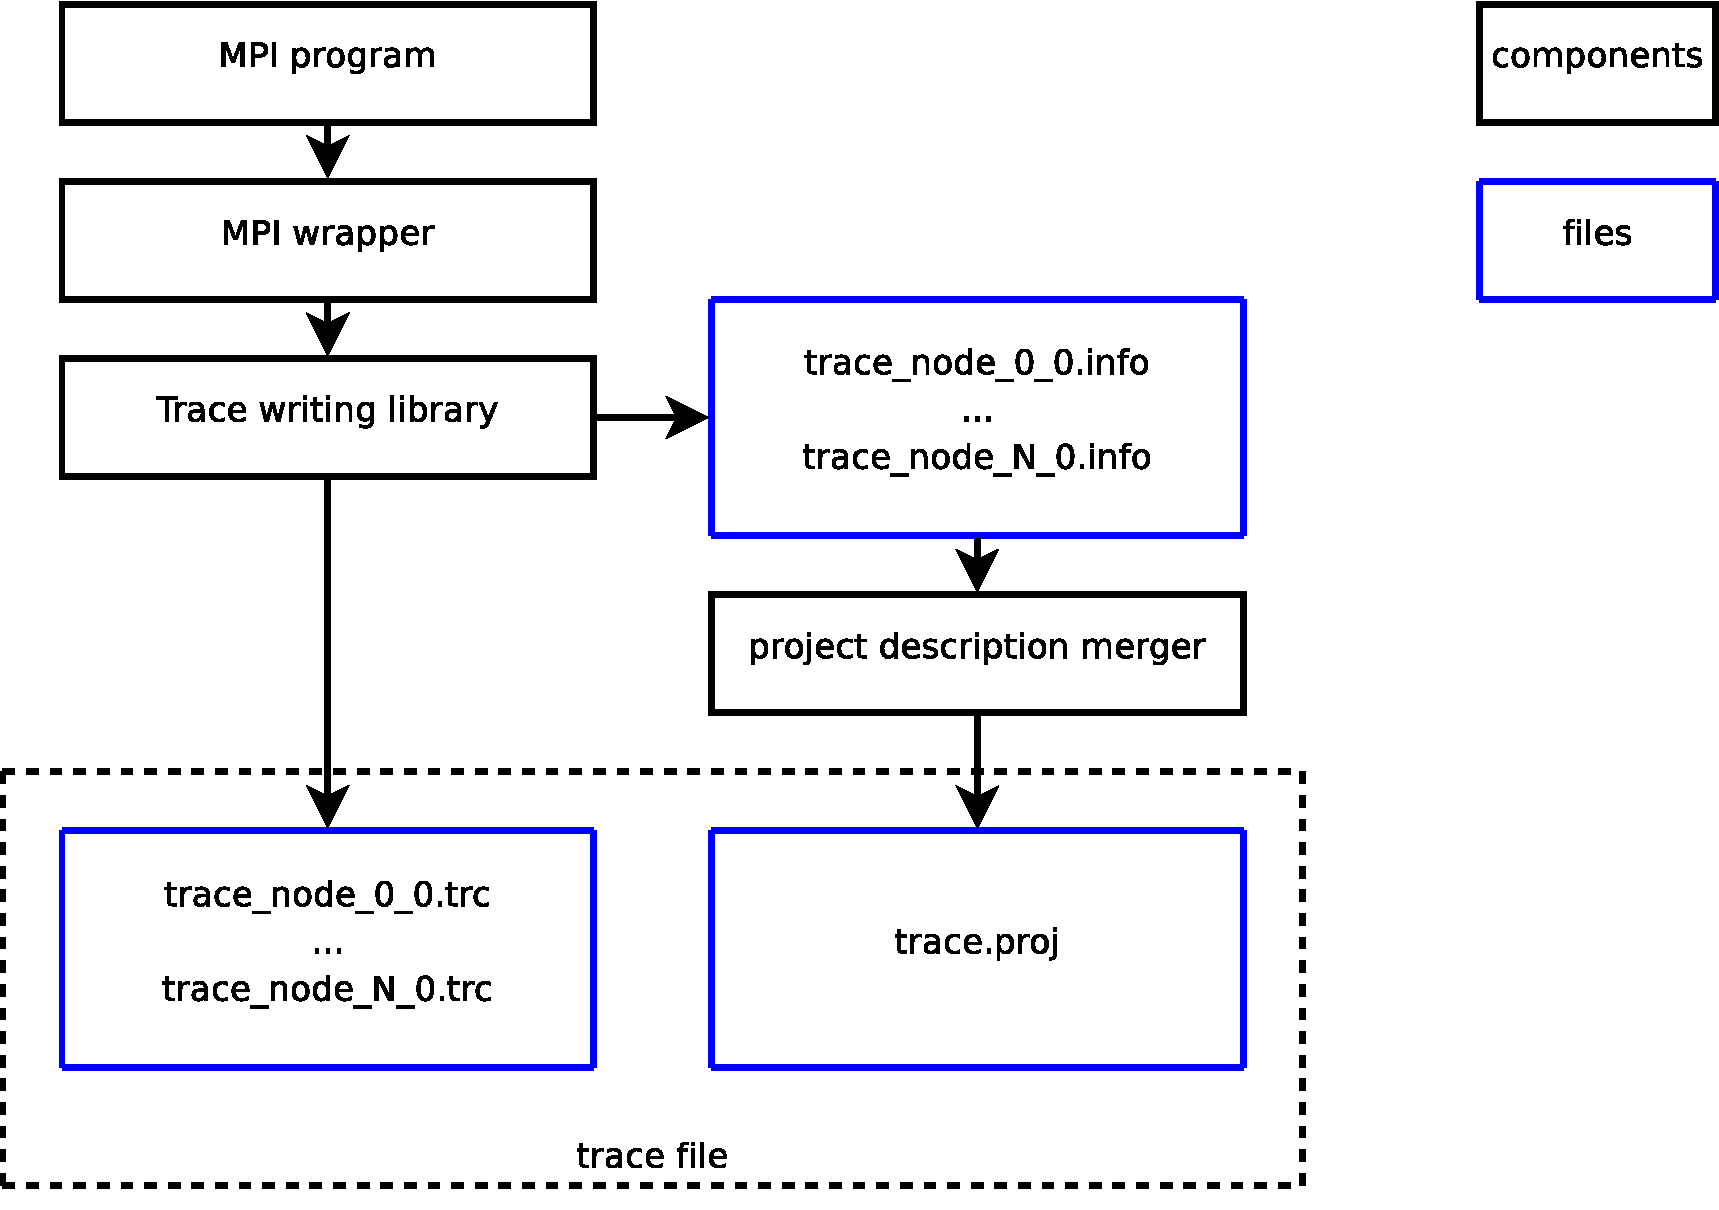
\includegraphics[width=0.93\textwidth]{img/dataflow-praes}
  \end{block}
\end{frame}

\subsection{HDTraceWritingCLibrary}
\begin{frame}[fragile]
  \begin{block}{HDTraceWritingCLibrary}
    \begin{itemize}
      \item management of the .info file
      \item management of the .trc log file
      \item abstraction layer for writing .trc xml log
      \item ensure correct syntax
      \item log correct time using \lstinline{gettimeofday()}
    \end{itemize}
  \end{block}

  \begin{block}{.info file}
    Information that needs to go into the project description.
  \end{block}
\end{frame}

\begin{frame}[fragile]
  \begin{block}{writing the xml trace}
    \begin{itemize}
    \item opening a trace structure
\begin{lstlisting}
hdTrace trace = hdT_createTrace(node, topology);
\end{lstlisting}
    \item logging a state with attributes and elements
\begin{lstlisting}
hdT_logStateStart(trace, "StateName");
hdT_logAttributes(trace, "cid='%d', comm_id)
hdT_logElement(trace, "Info", "key='%s' value='%s'", key, value);
hdT_logStateEnd(trace);
\end{lstlisting}
    \item closing the trace structure
\begin{lstlisting}
hdT_finalize(trace);
\end{lstlisting}
    \end{itemize}
  \end{block}
\end{frame}

\begin{frame}[fragile]
  \begin{block}{sample output (.trc file)}
\begin{lstlisting}
<Program rank='0' thread='0'>
...
<Barrier cid='1'  time='1240837588.806989' end='1240837588.806991'  />
<File_read fid='0' offset='0' size='16777216' count='16777216' tid='1275068673'  time='1240837588.806994' end='1240837588.816631'  />
<File_close fid='0'  time='1240837588.816638' end='1240837588.816657'  />
<Allreduce size='8' cid='1' count='1' tid='1275070475'
time='1240837588.816659' end='1240837588.816692'  />
...
</Program>
\end{lstlisting}

  \end{block}
\end{frame}


\begin{frame}[fragile]
  \begin{block}{nested calls}
    \begin{itemize}
    \item What if an MPI function is implemented using other MPI
      functions?
    \end{itemize}
  \end{block}
  \begin{block}{writing the xml trace}
    \begin{itemize}
    \item logging nested functions:
\begin{lstlisting}
hdT_logStateStart(trace, "A");
// log attributes, elements of state A 

  hdT_logStateStart(trace, "B");
  // log attributes, elements of state B 
  hdT_logStateEnd(trace);

hdT_logStateEnd(trace);
\end{lstlisting}
    \end{itemize}
  \end{block}
\end{frame}

\begin{frame}[fragile]
  \begin{block}{sample output for nested calls (.trc file)}
\begin{lstlisting}
<Nested>
  <inner_mpi_function ... />
</Nested>
<outer_function ... />
\end{lstlisting}
  \end{block}
\end{frame}


\begin{frame}[fragile]
  \begin{block}{.info files}
    \begin{itemize}
    \item syntax for writing to the info file:
\begin{lstlisting}
hdT_writeInfo(trace, format_string, ...);
\end{lstlisting}
    \item no further formatting, simple writing.
    \end{itemize}
  \end{block}
\end{frame}

\begin{frame}
  \begin{block}{HDTraceWritingCLibrary}
    Also in the trace writing library (Stephan): 
    \begin{itemize}
    \item statistics writing library
    \item topology library
    \end{itemize}
  \end{block}
\end{frame}

\subsection{HDMPIwrapper}

\begin{frame}[fragile]
  \begin{block}{HDMPIwrapper library}
    Task: Intercept MPI calls, log them 
  \end{block}
  \begin{block}{Method}
    \begin{itemize}
    \item Create a static library that defines certain MPI
      functions.  
    \item Link the library to an MPI program
    \item wrapper functions hide the original functions
    \item (Note: the wrapper depends on the implementation specific
      include files)
    \end{itemize}
  \end{block}
  \begin{block}{How is the call passed to MPI?}
    \begin{itemize}
    \item MPI implementation: every function defined twice:
    \item \lstinline{MPI_} prefix
    \item \lstinline{PMPI_} prefix
    \item $\to$ hide the \lstinline{MPI_} function and call the
      \lstinline{PMPI_} function
    \item (if a program uses PMPI functions, the wrapper won't work)
    \end{itemize}
  \end{block}
\end{frame}

\begin{frame}[fragile]
  \begin{block}{typical wrapper function}
\begin{lstlisting}
int MPI_Send(Type1 v1, ..., TypeN vN)
{
  int ret;
  hdT_logStateStart(trace, "Send");
  ret = PMPI_Send(v1,  v2,  v3,  v4,  v5,  v6);
  hdT_logAttributes(/* attributes */);
  hdT_logStateEnd(trace);
  return ret;
}
\end{lstlisting}
\end{block}
\begin{block}{}
  \begin{itemize}
  \item Redundant structure $\to$ generate wrapper functions using a
    script
  \item Adjustable: attributes and elements, which function to log 
  \end{itemize}
\end{block}
\end{frame}

\subsection{Project Description Merger}
\begin{frame}
  \begin{block}{reminder}
    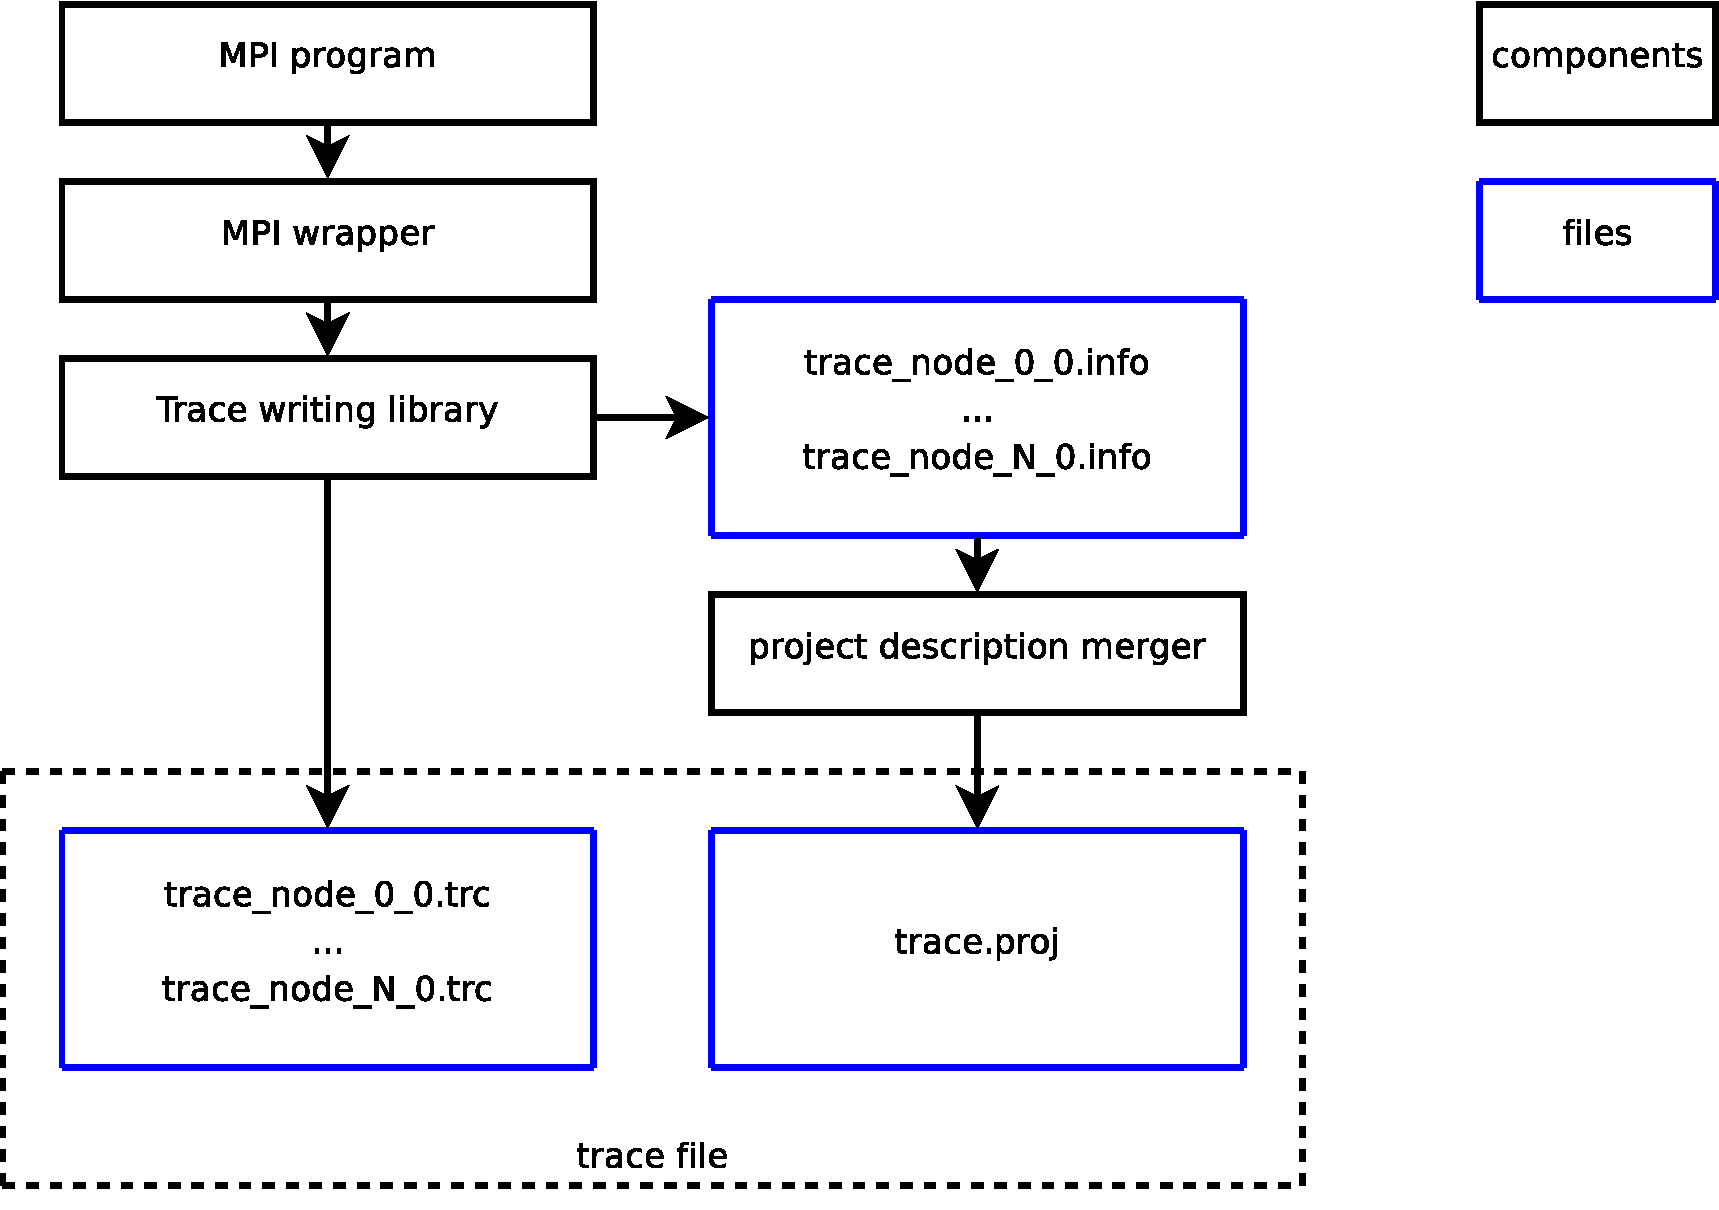
\includegraphics[width=0.93\textwidth]{img/dataflow-praes}
  \end{block}
\end{frame}

\begin{frame}
  \begin{block}{At program runtime}
    \begin{itemize}
      \item Trace writing library + MPI wrapper produces complete .trc
      files.
      \item project description file: created after the execution.
    \end{itemize}
  \end{block}
  \begin{block}{Project Description Merger}
    Python script that produces a project description file using the .info files.
  \end{block}
\end{frame}

\begin{frame}
  \begin{block}{What is stored in the project file}

    \begin{description}
    \item[Topology] Which log files belong to the
      trace?
    \item[File list] Which files are used and how are they called by
      different processes?
    \item[Communicator list] Which communicators are used and how are
      they called by different processes?
    \item[Datatypes] Which datatypes are used?
    \end{description}
  \end{block}
  \begin{block}{}
    \begin{itemize}
    \item Format: xml
    \end{itemize}
  \end{block}
\end{frame}

\section{Concepts}
\subsection{Topology}

\begin{frame}[fragile]
  \begin{block}{Topology}
    \begin{itemize}
    \item For program traces, the topology is given by $(\text{hostname},
      \text{rank}, \text{thread}) $
    \item Naming of the project file:
\begin{lstlisting}
<program name>.proj
\end{lstlisting}
    \item Naming of the trace files:
\begin{lstlisting}
<program name>_<hostname>_<rank>_<thread>.trc
\end{lstlisting}
    \end{itemize}
  \end{block}
\end{frame}

\begin{frame}[fragile]
  \begin{block}{project description file}
\begin{lstlisting}
<Topology>
 <Level name="Hostname">
  <Level name="Rank">
   <Level name="Thread">
   </Level>
  </Level>
 </Level>
 <Label value="node01">
  <Label value="1">
   <Label value="0" />
  </Label>
  <Label value="0">
   <Label value="0" />
  </Label>
 </Label>
</Topology>
\end{lstlisting}
  \end{block}
\end{frame}

\subsection{Files}
\begin{frame}[fragile]
  \begin{block}{Operations on files}
      open, close, delete, access
  \end{block}
  \begin{block}{Project description file}
    List the filename and its initial size.
  \end{block}
  \begin{block}{Wrapper}
    \begin{itemize}
    \item assign ID on first access via filename
    \item use hash map to store name $\leftrightarrow$ id relationship
    \item the file is always referred to via the id:
\begin{lstlisting}[emph={name,fid},emphstyle=\bf]
<File_open cid='0' name='filetest_02.tmp' flags='4' fid='1' ... />
<File_write_at_all fid='1' offset='0' size='1' count='1' tid='1275068673'  .../>
\end{lstlisting}
    \end{itemize}
  \end{block}
\end{frame}

\subsection{Communicators}
\begin{frame}[fragile]
  \begin{block}{communicators}
    \begin{itemize}
      \item assign id on first access
      \item need to know global rank $\leftrightarrow$ local rank map
        and id that is used by every rank
    \end{itemize}
  \end{block}
  \begin{block}{.trc file}
\begin{lstlisting}[emph={cid},emphstyle=\bf]
<File_open cid='0' name='filetest_02.tmp' ... />
\end{lstlisting}
  \end{block}
  \begin{block}{project file}
\begin{lstlisting}[emph={global,cid,local},emphstyle=\bf]
<CommunicatorList>
  <Communicator name="">
   <Rank global="1" local="1" cid="1" />
   <Rank global="2" local="0" cid="2" />
  </Communicator>
...
\end{lstlisting}
  \end{block}
\end{frame}

\subsection{Datatypes}
\begin{frame}[fragile]
  \begin{block}{Datatypes}
    \begin{itemize}
    \item Also referring to datatypes via process-internal id
    \item Problem: combined datatypes
    \item Solution: recursive unwrapping of datatypes using
\begin{lstlisting}
MPI_Type_get_envelope
MPI_Type_get_contents
\end{lstlisting}
    \item every process has its own datatype definitions
    \end{itemize}
  \end{block}
  \begin{block}{project file representation}
\begin{lstlisting}
<NAMED id="1275069445" name="MPI_INT"  />
<VECTOR id="-872415229" name="" count="5" blocklength="6" stride="7" oldType="1275069445"  />   
\end{lstlisting}
  \end{block}
\end{frame}

\subsection{Non-blocking Requests}
\begin{frame}[fragile]
  \begin{block}{Non-blocking requests}
    \begin{itemize}
    \item \lstinline{MPI_I*}-Functions return a request structure that
      can be used to wait for completion etc.
    \item split collective (\lstinline{*_begin} ... \lstinline{*_end})
      calls. (Maximum of one open split collective operation per file handle)
    \end{itemize}
  \end{block}
  \begin{block}{}
    \begin{itemize}
    \item Assign an id to every used \lstinline{MPI_Request} and
      \lstinline{MPI_File} 
    \item \lstinline{*_end} functions are transformed to
      \lstinline{Wait}s for the corresponding request.
    \end{itemize}
  \end{block}
\end{frame}

\begin{frame}[fragile]
  \begin{block}{non-blocking}
\begin{lstlisting}[emph={rid},emphstyle=\bf]
<Isend size='1' count='1' tid='1275068673' toRank='2' toTag='0' cid='0' rid='2' ... />
<Wait ... >
  <For rid='2' />
</Wait>
\end{lstlisting}

  \end{block}
  \begin{block}{split collective}
\begin{lstlisting}[emph={rid},emphstyle=\bf]
<File_write_at_all_begin fid='1' rid='0' ...  />
<Wait ... >
  <For rid='0' />
</Wait>
\end{lstlisting}
  \end{block}

\end{frame}

\section{Future Work}

\begin{frame}
  \begin{block}{Future Work}
    \begin{itemize}
    \item support threaded programs
    \item performance analysis
    \item synchronisation of timestamps
    \end{itemize}
  \end{block}
\end{frame}



\end{document}}